%!TEX root = mainfile.tex

\subsection{Observing Strategy for Redshift 6--8.5} % (fold)
\label{sec:observing_strategy_for_redshift_6_8}
	Due to their filters, Figure~\ref{fig:JWST_NIRspec_filters}, James Webb Space Telescope and E-ELT were considered for the survey used to observe galaxies between a redshift of 6 and 8.5. Both had the ability to do the colour photometry needed to identify the high redshift candidates. E-ELT had a larger field of view, and a larger primary mirror, but James Webb was able to resolve faint objects faster due to its low background. The following section outlines the motivation behind the choice of telescope for this survey.
	\begin{figure}[!htbp]
		\centering
			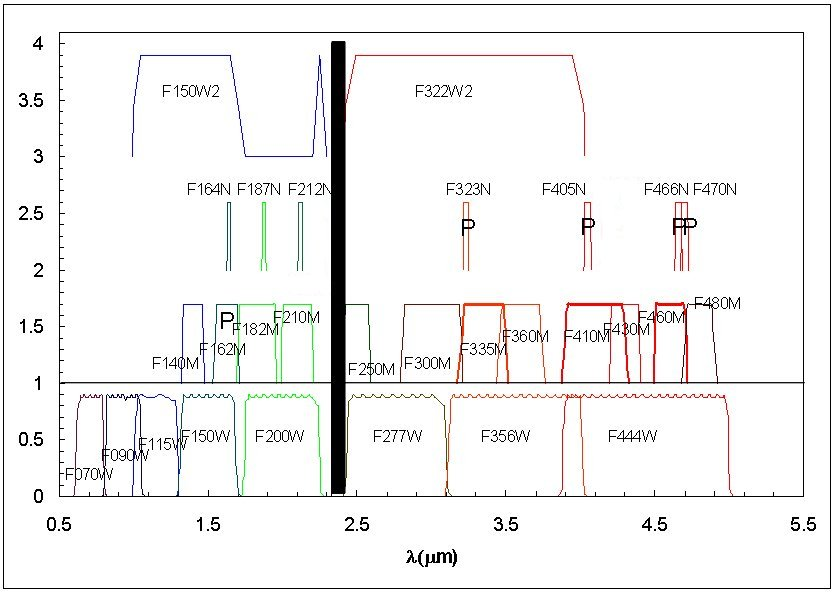
\includegraphics[width=0.7\textwidth]{../Images/JWST_NIRspec_filters.jpeg}
		\caption{\label{fig:JWST_NIRspec_filters}}
	\end{figure}

	\subsubsection{Results for E-ELT} % (fold)
	\label{sub:results_for_e_elt}
		Table 1 shows the number of galaxies observable for survey times of 0.1, 0.2, and 0.5\,million seconds. The number of galaxies that would be observed at different magnitudes is presented, and the table also displays the time taken to observe 1\,FoV down to each magnitude, and the number of galaxies in that field of view. The red number indicates how many FoVs were possible given the set total observing time. N/A indicates that there were either no galaxies at this magnitude, or that the time taken to get to this magnitude was larger than the intended total survey time. The total number of galaxies is also plotted against the magnitude in Figure~\ref{tab:galaxies_for_set_total_observing_time}.
		\begin{table}[!htbp]
			\begin{center}
				\begin{tabular}{c|c|>{\centering\arraybackslash}m{2.3cm}|c|c|c}
					\multirow{2}{*}{Magnitude} & \multirow{2}{*}{Time for 1 FoV} & No. of galaxies & \multicolumn{3}{|c}{Galaxies in total observing time of} \\
					\cline{4-6}
					 & & per FoV & 0.1mil & 0.2mil & 0.5mil\\
					 \hline\hline
					27 		& \num{2.35e3} 	& 0.06 		& $2\pm 0.3$ (42) 	& $5\pm 0.5$ (85) 	& $12\pm 0.8$ (212) \\
					28 		& \num{1.48e4} 	& 4.45 		& $26\pm 11$ (6) 	& $57\pm 16$ (13) 	& $146\pm 25$ (33) \\
					28.5 	& \num{3.72e4} 	& 18.27 	& $36\pm 25$ (2) 	& $91\pm 40$ (5) 	& $237\pm 65$ (13) \\
					29 		& \num{9.34e4} 	& 55.96 	& $56\pm 56$ (1) 	& $111\pm 78$ (2) 	& $279\pm 124$ (5) \\
					29.5 	& \num{2.32e5} 	& 139.04 	& N/A 				& N/A 				& $278\pm 276$ (1) \\
					30 		& \num{5.89e5} 	& 296.93 	& N/A 				& N/A 				& N/A
				\end{tabular}
			\end{center}
			\caption{Number of galaxies for set total observing time given different magnitudes/ survey areas.\label{tab:galaxies_for_set_total_observing_time}}
		\end{table}

		The program predicts that the total number of galaxies will be highest between a magnitude of 29 and 29.5. For a survey of 0.1\,million seconds per filter, it would be expected that a maximum of around 55 galaxies would be found, but this would have a large error due to cosmic variance. If the survey time was doubled, this number would be increased to around 111 galaxies, with 2 pointings and therefore slightly reduced cosmic variance. With a total exposure length of 0.5\,million seconds, and 1 pointing at 29.5\,mag, the maximum number of galaxies peaked at around 280, but 230 would be expected with 13 pointings and thus with smaller errors. The errors of the data due to cosmic variance are too large to plot clearly, and so the error has simply been included as a number in the table.
		\begin{figure}[!htbp]
			\centering
				\begingroup\endlinechar=-1
					\resizebox{0.8\textwidth}{!}{%
						% GNUPLOT: LaTeX picture with Postscript
\begingroup
  \makeatletter
  \providecommand\color[2][]{%
    \GenericError{(gnuplot) \space\space\space\@spaces}{%
      Package color not loaded in conjunction with
      terminal option `colourtext'%
    }{See the gnuplot documentation for explanation.%
    }{Either use 'blacktext' in gnuplot or load the package
      color.sty in LaTeX.}%
    \renewcommand\color[2][]{}%
  }%
  \providecommand\includegraphics[2][]{%
    \GenericError{(gnuplot) \space\space\space\@spaces}{%
      Package graphicx or graphics not loaded%
    }{See the gnuplot documentation for explanation.%
    }{The gnuplot epslatex terminal needs graphicx.sty or graphics.sty.}%
    \renewcommand\includegraphics[2][]{}%
  }%
  \providecommand\rotatebox[2]{#2}%
  \@ifundefined{ifGPcolor}{%
    \newif\ifGPcolor
    \GPcolortrue
  }{}%
  \@ifundefined{ifGPblacktext}{%
    \newif\ifGPblacktext
    \GPblacktexttrue
  }{}%
  % define a \g@addto@macro without @ in the name:
  \let\gplgaddtomacro\g@addto@macro
  % define empty templates for all commands taking text:
  \gdef\gplbacktext{}%
  \gdef\gplfronttext{}%
  \makeatother
  \ifGPblacktext
    % no textcolor at all
    \def\colorrgb#1{}%
    \def\colorgray#1{}%
  \else
    % gray or color?
    \ifGPcolor
      \def\colorrgb#1{\color[rgb]{#1}}%
      \def\colorgray#1{\color[gray]{#1}}%
      \expandafter\def\csname LTw\endcsname{\color{white}}%
      \expandafter\def\csname LTb\endcsname{\color{black}}%
      \expandafter\def\csname LTa\endcsname{\color{black}}%
      \expandafter\def\csname LT0\endcsname{\color[rgb]{1,0,0}}%
      \expandafter\def\csname LT1\endcsname{\color[rgb]{0,1,0}}%
      \expandafter\def\csname LT2\endcsname{\color[rgb]{0,0,1}}%
      \expandafter\def\csname LT3\endcsname{\color[rgb]{1,0,1}}%
      \expandafter\def\csname LT4\endcsname{\color[rgb]{0,1,1}}%
      \expandafter\def\csname LT5\endcsname{\color[rgb]{1,1,0}}%
      \expandafter\def\csname LT6\endcsname{\color[rgb]{0,0,0}}%
      \expandafter\def\csname LT7\endcsname{\color[rgb]{1,0.3,0}}%
      \expandafter\def\csname LT8\endcsname{\color[rgb]{0.5,0.5,0.5}}%
    \else
      % gray
      \def\colorrgb#1{\color{black}}%
      \def\colorgray#1{\color[gray]{#1}}%
      \expandafter\def\csname LTw\endcsname{\color{white}}%
      \expandafter\def\csname LTb\endcsname{\color{black}}%
      \expandafter\def\csname LTa\endcsname{\color{black}}%
      \expandafter\def\csname LT0\endcsname{\color{black}}%
      \expandafter\def\csname LT1\endcsname{\color{black}}%
      \expandafter\def\csname LT2\endcsname{\color{black}}%
      \expandafter\def\csname LT3\endcsname{\color{black}}%
      \expandafter\def\csname LT4\endcsname{\color{black}}%
      \expandafter\def\csname LT5\endcsname{\color{black}}%
      \expandafter\def\csname LT6\endcsname{\color{black}}%
      \expandafter\def\csname LT7\endcsname{\color{black}}%
      \expandafter\def\csname LT8\endcsname{\color{black}}%
    \fi
  \fi
  \setlength{\unitlength}{0.0500bp}%
  \begin{picture}(7200.00,4320.00)%
    \gplgaddtomacro\gplbacktext{%
      \put(747,595){\makebox(0,0)[r]{\strut{} 0}}%
      \put(747,1182){\makebox(0,0)[r]{\strut{} 50}}%
      \put(747,1768){\makebox(0,0)[r]{\strut{} 100}}%
      \put(747,2355){\makebox(0,0)[r]{\strut{} 150}}%
      \put(747,2942){\makebox(0,0)[r]{\strut{} 200}}%
      \put(747,3528){\makebox(0,0)[r]{\strut{} 250}}%
      \put(747,4115){\makebox(0,0)[r]{\strut{} 300}}%
      \put(849,409){\makebox(0,0){\strut{} 26.5}}%
      \put(1712,409){\makebox(0,0){\strut{} 27}}%
      \put(2576,409){\makebox(0,0){\strut{} 27.5}}%
      \put(3439,409){\makebox(0,0){\strut{} 28}}%
      \put(4303,409){\makebox(0,0){\strut{} 28.5}}%
      \put(5166,409){\makebox(0,0){\strut{} 29}}%
      \put(6030,409){\makebox(0,0){\strut{} 29.5}}%
      \put(6893,409){\makebox(0,0){\strut{} 30}}%
      \csname LTb\endcsname%
      \put(144,2355){\rotatebox{-270}{\makebox(0,0){\strut{}Number of Galaxies}}}%
      \csname LTb\endcsname%
      \put(3871,130){\makebox(0,0){\strut{}Magnitude ($M$)}}%
      \put(3871,4022){\makebox(0,0){\strut{}}}%
    }%
    \gplgaddtomacro\gplfronttext{%
      \csname LTb\endcsname%
      \put(2235,3729){\makebox(0,0)[r]{\strut{}\SI{0.1e6}{\second}}}%
      \csname LTb\endcsname%
      \put(2235,3543){\makebox(0,0)[r]{\strut{}\SI{0.2e6}{\second}}}%
      \csname LTb\endcsname%
      \put(2235,3357){\makebox(0,0)[r]{\strut{}\SI{0.5e6}{\second}}}%
    }%
    \gplbacktext
    \put(0,0){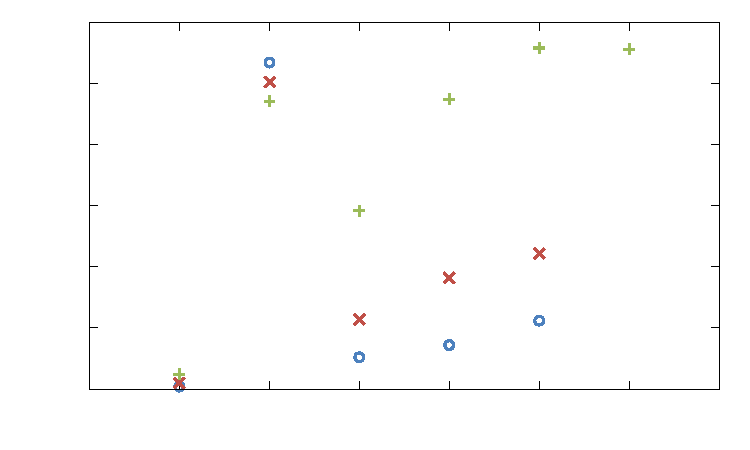
\includegraphics{GRAPH_Mag_vs_galaxies_in_time}}%
    \gplfronttext
  \end{picture}%
\endgroup

					}\endgroup
			\caption{Number of galaxies expected for different magnitudes, given set overall observing time (E-ELT 6--8.5).\label{fig:alpha_evolution}}
		\end{figure}

		The data for E-ELT was then compared to JWST for the same magnitudes and survey times to decide which telescope would be better equipped to find galaxies in this redshift range.
	% subsection results_for_e_elt (end)

	\subsubsection{Comparison} % (fold)
	\label{sub:comparison}
		The number of galaxies at each magnitude was plotted for both James Webb and E-ELT. Figure~\ref{fig:GRAPH_Mag_vs_galaxies_JWST_ELT_05} shows the comparison for the two telescopes each with the shutter open for 0.1 million seconds. Figure~\ref{fig:GRAPH_Mag_vs_galaxies_JWST_ELT_10} then displays the equivalent result but for a total time of 0.5\,million seconds.
		% \begin{figure}[!htbp]
  %       	\begin{minipage}[c]{0.8\linewidth}
		% 		\centering
		% 			\begingroup\endlinechar=-1
		% 				\resizebox{\textwidth}{!}{%
		% 					% GNUPLOT: LaTeX picture with Postscript
\begingroup
  \makeatletter
  \providecommand\color[2][]{%
    \GenericError{(gnuplot) \space\space\space\@spaces}{%
      Package color not loaded in conjunction with
      terminal option `colourtext'%
    }{See the gnuplot documentation for explanation.%
    }{Either use 'blacktext' in gnuplot or load the package
      color.sty in LaTeX.}%
    \renewcommand\color[2][]{}%
  }%
  \providecommand\includegraphics[2][]{%
    \GenericError{(gnuplot) \space\space\space\@spaces}{%
      Package graphicx or graphics not loaded%
    }{See the gnuplot documentation for explanation.%
    }{The gnuplot epslatex terminal needs graphicx.sty or graphics.sty.}%
    \renewcommand\includegraphics[2][]{}%
  }%
  \providecommand\rotatebox[2]{#2}%
  \@ifundefined{ifGPcolor}{%
    \newif\ifGPcolor
    \GPcolortrue
  }{}%
  \@ifundefined{ifGPblacktext}{%
    \newif\ifGPblacktext
    \GPblacktexttrue
  }{}%
  % define a \g@addto@macro without @ in the name:
  \let\gplgaddtomacro\g@addto@macro
  % define empty templates for all commands taking text:
  \gdef\gplbacktext{}%
  \gdef\gplfronttext{}%
  \makeatother
  \ifGPblacktext
    % no textcolor at all
    \def\colorrgb#1{}%
    \def\colorgray#1{}%
  \else
    % gray or color?
    \ifGPcolor
      \def\colorrgb#1{\color[rgb]{#1}}%
      \def\colorgray#1{\color[gray]{#1}}%
      \expandafter\def\csname LTw\endcsname{\color{white}}%
      \expandafter\def\csname LTb\endcsname{\color{black}}%
      \expandafter\def\csname LTa\endcsname{\color{black}}%
      \expandafter\def\csname LT0\endcsname{\color[rgb]{1,0,0}}%
      \expandafter\def\csname LT1\endcsname{\color[rgb]{0,1,0}}%
      \expandafter\def\csname LT2\endcsname{\color[rgb]{0,0,1}}%
      \expandafter\def\csname LT3\endcsname{\color[rgb]{1,0,1}}%
      \expandafter\def\csname LT4\endcsname{\color[rgb]{0,1,1}}%
      \expandafter\def\csname LT5\endcsname{\color[rgb]{1,1,0}}%
      \expandafter\def\csname LT6\endcsname{\color[rgb]{0,0,0}}%
      \expandafter\def\csname LT7\endcsname{\color[rgb]{1,0.3,0}}%
      \expandafter\def\csname LT8\endcsname{\color[rgb]{0.5,0.5,0.5}}%
    \else
      % gray
      \def\colorrgb#1{\color{black}}%
      \def\colorgray#1{\color[gray]{#1}}%
      \expandafter\def\csname LTw\endcsname{\color{white}}%
      \expandafter\def\csname LTb\endcsname{\color{black}}%
      \expandafter\def\csname LTa\endcsname{\color{black}}%
      \expandafter\def\csname LT0\endcsname{\color{black}}%
      \expandafter\def\csname LT1\endcsname{\color{black}}%
      \expandafter\def\csname LT2\endcsname{\color{black}}%
      \expandafter\def\csname LT3\endcsname{\color{black}}%
      \expandafter\def\csname LT4\endcsname{\color{black}}%
      \expandafter\def\csname LT5\endcsname{\color{black}}%
      \expandafter\def\csname LT6\endcsname{\color{black}}%
      \expandafter\def\csname LT7\endcsname{\color{black}}%
      \expandafter\def\csname LT8\endcsname{\color{black}}%
    \fi
  \fi
  \setlength{\unitlength}{0.0500bp}%
  \begin{picture}(7200.00,4320.00)%
    \gplgaddtomacro\gplbacktext{%
      \put(747,595){\makebox(0,0)[r]{\strut{} 0}}%
      \put(747,1182){\makebox(0,0)[r]{\strut{} 100}}%
      \put(747,1768){\makebox(0,0)[r]{\strut{} 200}}%
      \put(747,2355){\makebox(0,0)[r]{\strut{} 300}}%
      \put(747,2942){\makebox(0,0)[r]{\strut{} 400}}%
      \put(747,3528){\makebox(0,0)[r]{\strut{} 500}}%
      \put(747,4115){\makebox(0,0)[r]{\strut{} 600}}%
      \put(849,409){\makebox(0,0){\strut{} 26.5}}%
      \put(1712,409){\makebox(0,0){\strut{} 27}}%
      \put(2576,409){\makebox(0,0){\strut{} 27.5}}%
      \put(3439,409){\makebox(0,0){\strut{} 28}}%
      \put(4303,409){\makebox(0,0){\strut{} 28.5}}%
      \put(5166,409){\makebox(0,0){\strut{} 29}}%
      \put(6030,409){\makebox(0,0){\strut{} 29.5}}%
      \put(6893,409){\makebox(0,0){\strut{} 30}}%
      \csname LTb\endcsname%
      \put(144,2355){\rotatebox{-270}{\makebox(0,0){\strut{}Number of Galaxies}}}%
      \csname LTb\endcsname%
      \put(3871,130){\makebox(0,0){\strut{}Magnitude ($M$)}}%
      \put(3871,4022){\makebox(0,0){\strut{}}}%
    }%
    \gplgaddtomacro\gplfronttext{%
      \csname LTb\endcsname%
      \put(1890,3729){\makebox(0,0)[r]{\strut{}E-ELT}}%
      \csname LTb\endcsname%
      \put(1890,3543){\makebox(0,0)[r]{\strut{}JWST}}%
    }%
    \gplbacktext
    \put(0,0){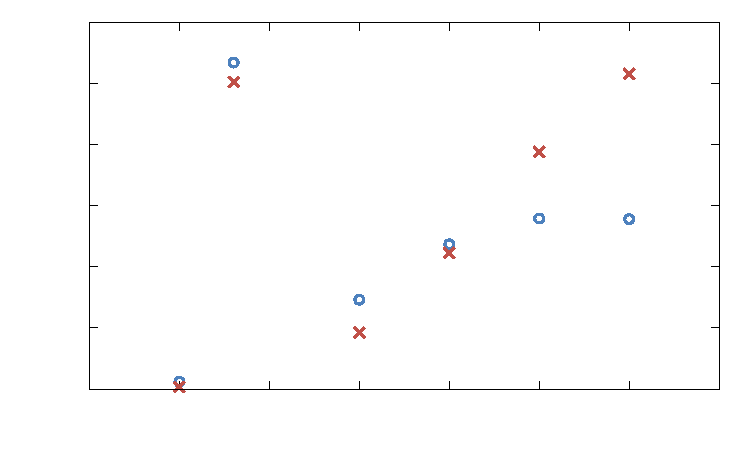
\includegraphics{GRAPH_Mag_vs_galaxies_JWST_ELT_05}}%
    \gplfronttext
  \end{picture}%
\endgroup

		% 				}\endgroup
		% 		\caption{Number of galaxies expected for different magnitudes, given set overall observing time (E-ELT 6--8.5).\label{fig:GRAPH_Mag_vs_galaxies_JWST_ELT_05}}
		% 	\end{minipage}
  %       	\begin{minipage}[c]{0.8\linewidth}
		% 		\centering
		% 			\begingroup\endlinechar=-1
		% 				\resizebox{\textwidth}{!}{%
		% 					% GNUPLOT: LaTeX picture with Postscript
\begingroup
  \makeatletter
  \providecommand\color[2][]{%
    \GenericError{(gnuplot) \space\space\space\@spaces}{%
      Package color not loaded in conjunction with
      terminal option `colourtext'%
    }{See the gnuplot documentation for explanation.%
    }{Either use 'blacktext' in gnuplot or load the package
      color.sty in LaTeX.}%
    \renewcommand\color[2][]{}%
  }%
  \providecommand\includegraphics[2][]{%
    \GenericError{(gnuplot) \space\space\space\@spaces}{%
      Package graphicx or graphics not loaded%
    }{See the gnuplot documentation for explanation.%
    }{The gnuplot epslatex terminal needs graphicx.sty or graphics.sty.}%
    \renewcommand\includegraphics[2][]{}%
  }%
  \providecommand\rotatebox[2]{#2}%
  \@ifundefined{ifGPcolor}{%
    \newif\ifGPcolor
    \GPcolortrue
  }{}%
  \@ifundefined{ifGPblacktext}{%
    \newif\ifGPblacktext
    \GPblacktexttrue
  }{}%
  % define a \g@addto@macro without @ in the name:
  \let\gplgaddtomacro\g@addto@macro
  % define empty templates for all commands taking text:
  \gdef\gplbacktext{}%
  \gdef\gplfronttext{}%
  \makeatother
  \ifGPblacktext
    % no textcolor at all
    \def\colorrgb#1{}%
    \def\colorgray#1{}%
  \else
    % gray or color?
    \ifGPcolor
      \def\colorrgb#1{\color[rgb]{#1}}%
      \def\colorgray#1{\color[gray]{#1}}%
      \expandafter\def\csname LTw\endcsname{\color{white}}%
      \expandafter\def\csname LTb\endcsname{\color{black}}%
      \expandafter\def\csname LTa\endcsname{\color{black}}%
      \expandafter\def\csname LT0\endcsname{\color[rgb]{1,0,0}}%
      \expandafter\def\csname LT1\endcsname{\color[rgb]{0,1,0}}%
      \expandafter\def\csname LT2\endcsname{\color[rgb]{0,0,1}}%
      \expandafter\def\csname LT3\endcsname{\color[rgb]{1,0,1}}%
      \expandafter\def\csname LT4\endcsname{\color[rgb]{0,1,1}}%
      \expandafter\def\csname LT5\endcsname{\color[rgb]{1,1,0}}%
      \expandafter\def\csname LT6\endcsname{\color[rgb]{0,0,0}}%
      \expandafter\def\csname LT7\endcsname{\color[rgb]{1,0.3,0}}%
      \expandafter\def\csname LT8\endcsname{\color[rgb]{0.5,0.5,0.5}}%
    \else
      % gray
      \def\colorrgb#1{\color{black}}%
      \def\colorgray#1{\color[gray]{#1}}%
      \expandafter\def\csname LTw\endcsname{\color{white}}%
      \expandafter\def\csname LTb\endcsname{\color{black}}%
      \expandafter\def\csname LTa\endcsname{\color{black}}%
      \expandafter\def\csname LT0\endcsname{\color{black}}%
      \expandafter\def\csname LT1\endcsname{\color{black}}%
      \expandafter\def\csname LT2\endcsname{\color{black}}%
      \expandafter\def\csname LT3\endcsname{\color{black}}%
      \expandafter\def\csname LT4\endcsname{\color{black}}%
      \expandafter\def\csname LT5\endcsname{\color{black}}%
      \expandafter\def\csname LT6\endcsname{\color{black}}%
      \expandafter\def\csname LT7\endcsname{\color{black}}%
      \expandafter\def\csname LT8\endcsname{\color{black}}%
    \fi
  \fi
  \setlength{\unitlength}{0.0500bp}%
  \begin{picture}(7200.00,4320.00)%
    \gplgaddtomacro\gplbacktext{%
      \put(747,595){\makebox(0,0)[r]{\strut{} 0}}%
      \put(747,1182){\makebox(0,0)[r]{\strut{} 20}}%
      \put(747,1768){\makebox(0,0)[r]{\strut{} 40}}%
      \put(747,2355){\makebox(0,0)[r]{\strut{} 60}}%
      \put(747,2942){\makebox(0,0)[r]{\strut{} 80}}%
      \put(747,3528){\makebox(0,0)[r]{\strut{} 100}}%
      \put(747,4115){\makebox(0,0)[r]{\strut{} 120}}%
      \put(849,409){\makebox(0,0){\strut{} 26.5}}%
      \put(1712,409){\makebox(0,0){\strut{} 27}}%
      \put(2576,409){\makebox(0,0){\strut{} 27.5}}%
      \put(3439,409){\makebox(0,0){\strut{} 28}}%
      \put(4303,409){\makebox(0,0){\strut{} 28.5}}%
      \put(5166,409){\makebox(0,0){\strut{} 29}}%
      \put(6030,409){\makebox(0,0){\strut{} 29.5}}%
      \put(6893,409){\makebox(0,0){\strut{} 30}}%
      \csname LTb\endcsname%
      \put(144,2355){\rotatebox{-270}{\makebox(0,0){\strut{}Number of Galaxies}}}%
      \csname LTb\endcsname%
      \put(3871,130){\makebox(0,0){\strut{}Magnitude ($M$)}}%
      \put(3871,4022){\makebox(0,0){\strut{}}}%
    }%
    \gplgaddtomacro\gplfronttext{%
      \csname LTb\endcsname%
      \put(1890,3729){\makebox(0,0)[r]{\strut{}E-ELT}}%
      \csname LTb\endcsname%
      \put(1890,3543){\makebox(0,0)[r]{\strut{}JWST}}%
    }%
    \gplbacktext
    \put(0,0){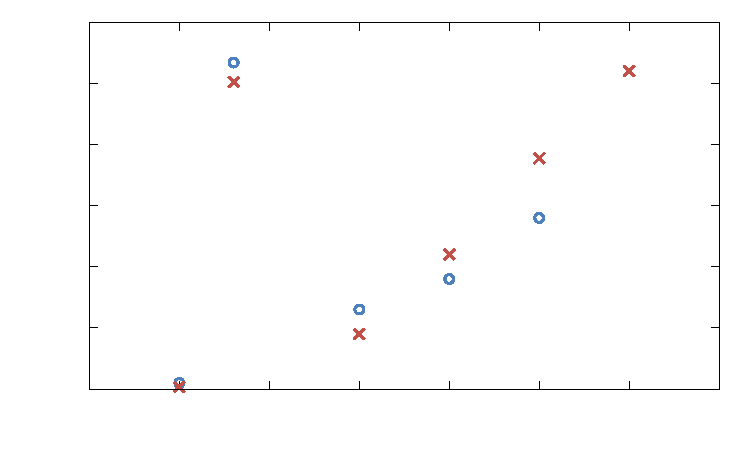
\includegraphics{GRAPH_Mag_vs_galaxies_JWST_ELT_10}}%
    \gplfronttext
  \end{picture}%
\endgroup

		% 				}\endgroup
		% 		\caption{Number of galaxies expected for different magnitudes, given set overall observing time (E-ELT 6--8.5).\label{fig:GRAPH_Mag_vs_galaxies_JWST_ELT_10}}
		% 	\end{minipage}
		% \end{figure}
		\begin{figure}[!htbp]
			\centering
				\begingroup\endlinechar=-1
					\resizebox{0.8\textwidth}{!}{%
						% GNUPLOT: LaTeX picture with Postscript
\begingroup
  \makeatletter
  \providecommand\color[2][]{%
    \GenericError{(gnuplot) \space\space\space\@spaces}{%
      Package color not loaded in conjunction with
      terminal option `colourtext'%
    }{See the gnuplot documentation for explanation.%
    }{Either use 'blacktext' in gnuplot or load the package
      color.sty in LaTeX.}%
    \renewcommand\color[2][]{}%
  }%
  \providecommand\includegraphics[2][]{%
    \GenericError{(gnuplot) \space\space\space\@spaces}{%
      Package graphicx or graphics not loaded%
    }{See the gnuplot documentation for explanation.%
    }{The gnuplot epslatex terminal needs graphicx.sty or graphics.sty.}%
    \renewcommand\includegraphics[2][]{}%
  }%
  \providecommand\rotatebox[2]{#2}%
  \@ifundefined{ifGPcolor}{%
    \newif\ifGPcolor
    \GPcolortrue
  }{}%
  \@ifundefined{ifGPblacktext}{%
    \newif\ifGPblacktext
    \GPblacktexttrue
  }{}%
  % define a \g@addto@macro without @ in the name:
  \let\gplgaddtomacro\g@addto@macro
  % define empty templates for all commands taking text:
  \gdef\gplbacktext{}%
  \gdef\gplfronttext{}%
  \makeatother
  \ifGPblacktext
    % no textcolor at all
    \def\colorrgb#1{}%
    \def\colorgray#1{}%
  \else
    % gray or color?
    \ifGPcolor
      \def\colorrgb#1{\color[rgb]{#1}}%
      \def\colorgray#1{\color[gray]{#1}}%
      \expandafter\def\csname LTw\endcsname{\color{white}}%
      \expandafter\def\csname LTb\endcsname{\color{black}}%
      \expandafter\def\csname LTa\endcsname{\color{black}}%
      \expandafter\def\csname LT0\endcsname{\color[rgb]{1,0,0}}%
      \expandafter\def\csname LT1\endcsname{\color[rgb]{0,1,0}}%
      \expandafter\def\csname LT2\endcsname{\color[rgb]{0,0,1}}%
      \expandafter\def\csname LT3\endcsname{\color[rgb]{1,0,1}}%
      \expandafter\def\csname LT4\endcsname{\color[rgb]{0,1,1}}%
      \expandafter\def\csname LT5\endcsname{\color[rgb]{1,1,0}}%
      \expandafter\def\csname LT6\endcsname{\color[rgb]{0,0,0}}%
      \expandafter\def\csname LT7\endcsname{\color[rgb]{1,0.3,0}}%
      \expandafter\def\csname LT8\endcsname{\color[rgb]{0.5,0.5,0.5}}%
    \else
      % gray
      \def\colorrgb#1{\color{black}}%
      \def\colorgray#1{\color[gray]{#1}}%
      \expandafter\def\csname LTw\endcsname{\color{white}}%
      \expandafter\def\csname LTb\endcsname{\color{black}}%
      \expandafter\def\csname LTa\endcsname{\color{black}}%
      \expandafter\def\csname LT0\endcsname{\color{black}}%
      \expandafter\def\csname LT1\endcsname{\color{black}}%
      \expandafter\def\csname LT2\endcsname{\color{black}}%
      \expandafter\def\csname LT3\endcsname{\color{black}}%
      \expandafter\def\csname LT4\endcsname{\color{black}}%
      \expandafter\def\csname LT5\endcsname{\color{black}}%
      \expandafter\def\csname LT6\endcsname{\color{black}}%
      \expandafter\def\csname LT7\endcsname{\color{black}}%
      \expandafter\def\csname LT8\endcsname{\color{black}}%
    \fi
  \fi
  \setlength{\unitlength}{0.0500bp}%
  \begin{picture}(7200.00,4320.00)%
    \gplgaddtomacro\gplbacktext{%
      \put(747,595){\makebox(0,0)[r]{\strut{} 0}}%
      \put(747,1182){\makebox(0,0)[r]{\strut{} 100}}%
      \put(747,1768){\makebox(0,0)[r]{\strut{} 200}}%
      \put(747,2355){\makebox(0,0)[r]{\strut{} 300}}%
      \put(747,2942){\makebox(0,0)[r]{\strut{} 400}}%
      \put(747,3528){\makebox(0,0)[r]{\strut{} 500}}%
      \put(747,4115){\makebox(0,0)[r]{\strut{} 600}}%
      \put(849,409){\makebox(0,0){\strut{} 26.5}}%
      \put(1712,409){\makebox(0,0){\strut{} 27}}%
      \put(2576,409){\makebox(0,0){\strut{} 27.5}}%
      \put(3439,409){\makebox(0,0){\strut{} 28}}%
      \put(4303,409){\makebox(0,0){\strut{} 28.5}}%
      \put(5166,409){\makebox(0,0){\strut{} 29}}%
      \put(6030,409){\makebox(0,0){\strut{} 29.5}}%
      \put(6893,409){\makebox(0,0){\strut{} 30}}%
      \csname LTb\endcsname%
      \put(144,2355){\rotatebox{-270}{\makebox(0,0){\strut{}Number of Galaxies}}}%
      \csname LTb\endcsname%
      \put(3871,130){\makebox(0,0){\strut{}Magnitude ($M$)}}%
      \put(3871,4022){\makebox(0,0){\strut{}}}%
    }%
    \gplgaddtomacro\gplfronttext{%
      \csname LTb\endcsname%
      \put(1890,3729){\makebox(0,0)[r]{\strut{}E-ELT}}%
      \csname LTb\endcsname%
      \put(1890,3543){\makebox(0,0)[r]{\strut{}JWST}}%
    }%
    \gplbacktext
    \put(0,0){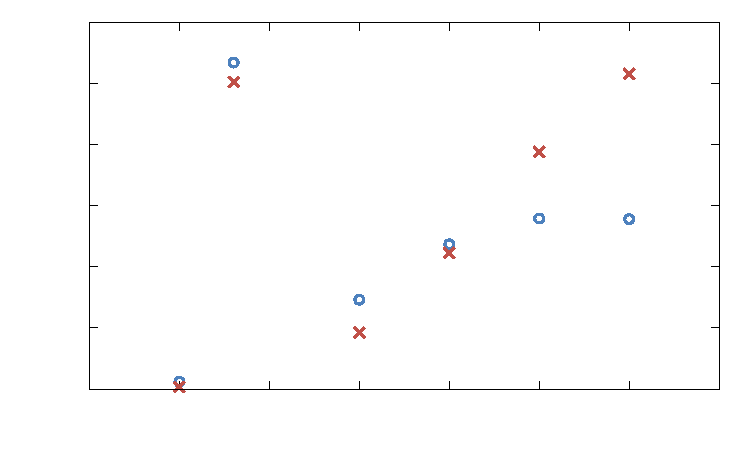
\includegraphics{GRAPH_Mag_vs_galaxies_JWST_ELT_05}}%
    \gplfronttext
  \end{picture}%
\endgroup

					}\endgroup
			\caption{Number of galaxies expected for different magnitudes, given set overall observing time (E-ELT 6--8.5).\label{fig:GRAPH_Mag_vs_galaxies_JWST_ELT_05}}
		\end{figure}
		\begin{figure}[!htbp]
			\centering
				\begingroup\endlinechar=-1
					\resizebox{0.8\textwidth}{!}{%
						% GNUPLOT: LaTeX picture with Postscript
\begingroup
  \makeatletter
  \providecommand\color[2][]{%
    \GenericError{(gnuplot) \space\space\space\@spaces}{%
      Package color not loaded in conjunction with
      terminal option `colourtext'%
    }{See the gnuplot documentation for explanation.%
    }{Either use 'blacktext' in gnuplot or load the package
      color.sty in LaTeX.}%
    \renewcommand\color[2][]{}%
  }%
  \providecommand\includegraphics[2][]{%
    \GenericError{(gnuplot) \space\space\space\@spaces}{%
      Package graphicx or graphics not loaded%
    }{See the gnuplot documentation for explanation.%
    }{The gnuplot epslatex terminal needs graphicx.sty or graphics.sty.}%
    \renewcommand\includegraphics[2][]{}%
  }%
  \providecommand\rotatebox[2]{#2}%
  \@ifundefined{ifGPcolor}{%
    \newif\ifGPcolor
    \GPcolortrue
  }{}%
  \@ifundefined{ifGPblacktext}{%
    \newif\ifGPblacktext
    \GPblacktexttrue
  }{}%
  % define a \g@addto@macro without @ in the name:
  \let\gplgaddtomacro\g@addto@macro
  % define empty templates for all commands taking text:
  \gdef\gplbacktext{}%
  \gdef\gplfronttext{}%
  \makeatother
  \ifGPblacktext
    % no textcolor at all
    \def\colorrgb#1{}%
    \def\colorgray#1{}%
  \else
    % gray or color?
    \ifGPcolor
      \def\colorrgb#1{\color[rgb]{#1}}%
      \def\colorgray#1{\color[gray]{#1}}%
      \expandafter\def\csname LTw\endcsname{\color{white}}%
      \expandafter\def\csname LTb\endcsname{\color{black}}%
      \expandafter\def\csname LTa\endcsname{\color{black}}%
      \expandafter\def\csname LT0\endcsname{\color[rgb]{1,0,0}}%
      \expandafter\def\csname LT1\endcsname{\color[rgb]{0,1,0}}%
      \expandafter\def\csname LT2\endcsname{\color[rgb]{0,0,1}}%
      \expandafter\def\csname LT3\endcsname{\color[rgb]{1,0,1}}%
      \expandafter\def\csname LT4\endcsname{\color[rgb]{0,1,1}}%
      \expandafter\def\csname LT5\endcsname{\color[rgb]{1,1,0}}%
      \expandafter\def\csname LT6\endcsname{\color[rgb]{0,0,0}}%
      \expandafter\def\csname LT7\endcsname{\color[rgb]{1,0.3,0}}%
      \expandafter\def\csname LT8\endcsname{\color[rgb]{0.5,0.5,0.5}}%
    \else
      % gray
      \def\colorrgb#1{\color{black}}%
      \def\colorgray#1{\color[gray]{#1}}%
      \expandafter\def\csname LTw\endcsname{\color{white}}%
      \expandafter\def\csname LTb\endcsname{\color{black}}%
      \expandafter\def\csname LTa\endcsname{\color{black}}%
      \expandafter\def\csname LT0\endcsname{\color{black}}%
      \expandafter\def\csname LT1\endcsname{\color{black}}%
      \expandafter\def\csname LT2\endcsname{\color{black}}%
      \expandafter\def\csname LT3\endcsname{\color{black}}%
      \expandafter\def\csname LT4\endcsname{\color{black}}%
      \expandafter\def\csname LT5\endcsname{\color{black}}%
      \expandafter\def\csname LT6\endcsname{\color{black}}%
      \expandafter\def\csname LT7\endcsname{\color{black}}%
      \expandafter\def\csname LT8\endcsname{\color{black}}%
    \fi
  \fi
  \setlength{\unitlength}{0.0500bp}%
  \begin{picture}(7200.00,4320.00)%
    \gplgaddtomacro\gplbacktext{%
      \put(747,595){\makebox(0,0)[r]{\strut{} 0}}%
      \put(747,1182){\makebox(0,0)[r]{\strut{} 20}}%
      \put(747,1768){\makebox(0,0)[r]{\strut{} 40}}%
      \put(747,2355){\makebox(0,0)[r]{\strut{} 60}}%
      \put(747,2942){\makebox(0,0)[r]{\strut{} 80}}%
      \put(747,3528){\makebox(0,0)[r]{\strut{} 100}}%
      \put(747,4115){\makebox(0,0)[r]{\strut{} 120}}%
      \put(849,409){\makebox(0,0){\strut{} 26.5}}%
      \put(1712,409){\makebox(0,0){\strut{} 27}}%
      \put(2576,409){\makebox(0,0){\strut{} 27.5}}%
      \put(3439,409){\makebox(0,0){\strut{} 28}}%
      \put(4303,409){\makebox(0,0){\strut{} 28.5}}%
      \put(5166,409){\makebox(0,0){\strut{} 29}}%
      \put(6030,409){\makebox(0,0){\strut{} 29.5}}%
      \put(6893,409){\makebox(0,0){\strut{} 30}}%
      \csname LTb\endcsname%
      \put(144,2355){\rotatebox{-270}{\makebox(0,0){\strut{}Number of Galaxies}}}%
      \csname LTb\endcsname%
      \put(3871,130){\makebox(0,0){\strut{}Magnitude ($M$)}}%
      \put(3871,4022){\makebox(0,0){\strut{}}}%
    }%
    \gplgaddtomacro\gplfronttext{%
      \csname LTb\endcsname%
      \put(1890,3729){\makebox(0,0)[r]{\strut{}E-ELT}}%
      \csname LTb\endcsname%
      \put(1890,3543){\makebox(0,0)[r]{\strut{}JWST}}%
    }%
    \gplbacktext
    \put(0,0){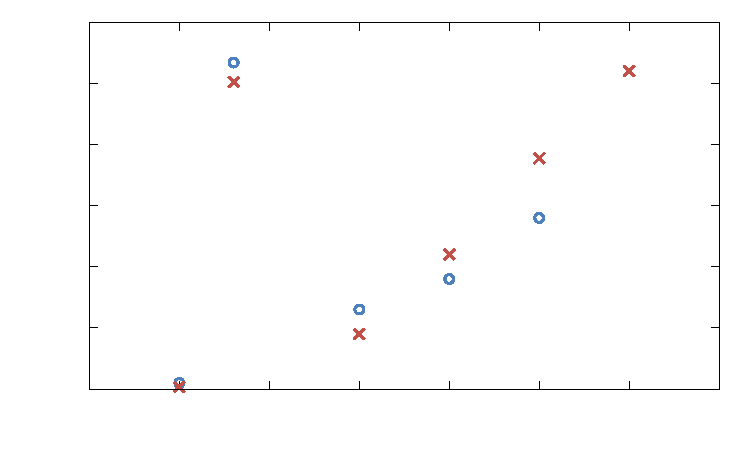
\includegraphics{GRAPH_Mag_vs_galaxies_JWST_ELT_10}}%
    \gplfronttext
  \end{picture}%
\endgroup

					}\endgroup
			\caption{Number of galaxies expected for different magnitudes, given set overall observing time (E-ELT 6--8.5).\label{fig:GRAPH_Mag_vs_galaxies_JWST_ELT_10}}
		\end{figure}

		The results indicate that James Webb would be able to observe more galaxies at higher magnitudes, with E-ELT peaking around 280 galaxies for 0.5\,million seconds, compared to JWST's 516 (and still increasing). In Figure~\ref{fig:GRAPH_Mag_vs_galaxies_JWST_ELT_10} it can be seen that for the 0.1\,million data set, although E-ELT is expected to observe more galaxies at lower magnitudes, James Webb produces the most promising result at a magnitude of 29.5. James Webb was therefore chosen over E-ELT to conduct the 6 to 8.5 redshift survey.
	% subsection comparison (end)

	\subsubsection{Detailed Results for JWST} % (fold)
	\label{sub:detailed_results_for_jwst}
		Table~\ref{tab:galaxies_for_set_total_observing_time_JWST} and figure~\ref{fig:galaxies_expected_JWST_6-8} 4 present the same information as shown for ELT, but instead using James Webb observing times and field of view.
		\begin{table}[!htbp]
			\begin{center}
				\begin{tabular}{c|c|>{\centering\arraybackslash}m{2.3cm}|c|c|c}
					\multirow{2}{*}{Mag} & \multirow{2}{*}{Time per FoV} & No. galaxies & \multicolumn{3}{|c}{Galaxies in total observing time of} \\
					\cline{4-6}
					 & & per FoV & 0.1mil & 0.2mil & 0.5mil\\
					 \hline\hline
27 		& \num{4.31e2} 	& 0.0029 	& $0.67\pm0.06$ (232) 	& $1.34\pm0.09$ (464) 	& $3.36 \pm0.14$ (1160) \\
28 		& \num{1.16e3} 	& 0.214 	& $18\pm2.67$ (86) 		& $36.81\pm3.85$ (172)	& $92.23\pm6.11$ (431) \\
28.5 	& \num{1.97e3} 	& 0.881 	& $44.05\pm 8.74$ (50) 	& $88.98\pm12.17$ (101) & $222.89\pm19.28$ (253) \\
29 		& \num{3.46e3} 	& 2.697 	& $75.52\pm19.63$ (28) 	& $153.73\pm27.99$ (57) & $388.37\pm44.51$ (144) \\
29.5 	& \num{6.44e3} 	& 6.702 	& $100.53\pm36.96$ (15) & $207.76\pm46.48$ (31) & $516.05\pm73.24$ (77) \\
30 		& \num{1.29e4} 	& 14.312 	& $100.18\pm52.07$ (7) 	& $214.68\pm76.32$ (15) & $543.86\pm121.34$ (38) \\
30.5 	& \num{2.78e4} 	& 27.380 	& $82.14\pm65.1$ (3) 	& $191.66\pm99.62$ (7) 	& $465.46\pm164.54$ (17) \\
31 		& \num{6.43e4} 	& 48.346 	& $48.35\pm66$ (1) 		& $145.04\pm115.15$ (3) & $388.42\pm201.9$ (7) \\
32 		& \num{3.8e5} 	& 128.461 	& N/A 					& N/A 					& $128.46\pm$ (1)
				\end{tabular}
			\end{center}
			\caption{Number of galaxies for set total observing time given different magnitudes/ survey areas for JWST.\label{tab:galaxies_for_set_total_observing_time_JWST}}
		\end{table}
		\begin{figure}[!htbp]
			\centering
				\begingroup\endlinechar=-1
					\resizebox{0.8\textwidth}{!}{%
						% GNUPLOT: LaTeX picture with Postscript
\begingroup
  \makeatletter
  \providecommand\color[2][]{%
    \GenericError{(gnuplot) \space\space\space\@spaces}{%
      Package color not loaded in conjunction with
      terminal option `colourtext'%
    }{See the gnuplot documentation for explanation.%
    }{Either use 'blacktext' in gnuplot or load the package
      color.sty in LaTeX.}%
    \renewcommand\color[2][]{}%
  }%
  \providecommand\includegraphics[2][]{%
    \GenericError{(gnuplot) \space\space\space\@spaces}{%
      Package graphicx or graphics not loaded%
    }{See the gnuplot documentation for explanation.%
    }{The gnuplot epslatex terminal needs graphicx.sty or graphics.sty.}%
    \renewcommand\includegraphics[2][]{}%
  }%
  \providecommand\rotatebox[2]{#2}%
  \@ifundefined{ifGPcolor}{%
    \newif\ifGPcolor
    \GPcolortrue
  }{}%
  \@ifundefined{ifGPblacktext}{%
    \newif\ifGPblacktext
    \GPblacktexttrue
  }{}%
  % define a \g@addto@macro without @ in the name:
  \let\gplgaddtomacro\g@addto@macro
  % define empty templates for all commands taking text:
  \gdef\gplbacktext{}%
  \gdef\gplfronttext{}%
  \makeatother
  \ifGPblacktext
    % no textcolor at all
    \def\colorrgb#1{}%
    \def\colorgray#1{}%
  \else
    % gray or color?
    \ifGPcolor
      \def\colorrgb#1{\color[rgb]{#1}}%
      \def\colorgray#1{\color[gray]{#1}}%
      \expandafter\def\csname LTw\endcsname{\color{white}}%
      \expandafter\def\csname LTb\endcsname{\color{black}}%
      \expandafter\def\csname LTa\endcsname{\color{black}}%
      \expandafter\def\csname LT0\endcsname{\color[rgb]{1,0,0}}%
      \expandafter\def\csname LT1\endcsname{\color[rgb]{0,1,0}}%
      \expandafter\def\csname LT2\endcsname{\color[rgb]{0,0,1}}%
      \expandafter\def\csname LT3\endcsname{\color[rgb]{1,0,1}}%
      \expandafter\def\csname LT4\endcsname{\color[rgb]{0,1,1}}%
      \expandafter\def\csname LT5\endcsname{\color[rgb]{1,1,0}}%
      \expandafter\def\csname LT6\endcsname{\color[rgb]{0,0,0}}%
      \expandafter\def\csname LT7\endcsname{\color[rgb]{1,0.3,0}}%
      \expandafter\def\csname LT8\endcsname{\color[rgb]{0.5,0.5,0.5}}%
    \else
      % gray
      \def\colorrgb#1{\color{black}}%
      \def\colorgray#1{\color[gray]{#1}}%
      \expandafter\def\csname LTw\endcsname{\color{white}}%
      \expandafter\def\csname LTb\endcsname{\color{black}}%
      \expandafter\def\csname LTa\endcsname{\color{black}}%
      \expandafter\def\csname LT0\endcsname{\color{black}}%
      \expandafter\def\csname LT1\endcsname{\color{black}}%
      \expandafter\def\csname LT2\endcsname{\color{black}}%
      \expandafter\def\csname LT3\endcsname{\color{black}}%
      \expandafter\def\csname LT4\endcsname{\color{black}}%
      \expandafter\def\csname LT5\endcsname{\color{black}}%
      \expandafter\def\csname LT6\endcsname{\color{black}}%
      \expandafter\def\csname LT7\endcsname{\color{black}}%
      \expandafter\def\csname LT8\endcsname{\color{black}}%
    \fi
  \fi
  \setlength{\unitlength}{0.0500bp}%
  \begin{picture}(7200.00,4320.00)%
    \gplgaddtomacro\gplbacktext{%
      \put(747,595){\makebox(0,0)[r]{\strut{} 0}}%
      \put(747,1182){\makebox(0,0)[r]{\strut{} 100}}%
      \put(747,1768){\makebox(0,0)[r]{\strut{} 200}}%
      \put(747,2355){\makebox(0,0)[r]{\strut{} 300}}%
      \put(747,2942){\makebox(0,0)[r]{\strut{} 400}}%
      \put(747,3528){\makebox(0,0)[r]{\strut{} 500}}%
      \put(747,4115){\makebox(0,0)[r]{\strut{} 600}}%
      \put(1353,409){\makebox(0,0){\strut{} 27}}%
      \put(2360,409){\makebox(0,0){\strut{} 28}}%
      \put(3367,409){\makebox(0,0){\strut{} 29}}%
      \put(4375,409){\makebox(0,0){\strut{} 30}}%
      \put(5382,409){\makebox(0,0){\strut{} 31}}%
      \put(6389,409){\makebox(0,0){\strut{} 32}}%
      \csname LTb\endcsname%
      \put(144,2355){\rotatebox{-270}{\makebox(0,0){\strut{}Number of Galaxies}}}%
      \csname LTb\endcsname%
      \put(3871,130){\makebox(0,0){\strut{}Magnitude ($M$)}}%
      \put(3871,4022){\makebox(0,0){\strut{}}}%
    }%
    \gplgaddtomacro\gplfronttext{%
      \csname LTb\endcsname%
      \put(2178,3729){\makebox(0,0)[r]{\strut{}\SI{0.1e6}{\second}}}%
      \csname LTb\endcsname%
      \put(2178,3543){\makebox(0,0)[r]{\strut{}\SI{0.2e6}{\second}}}%
      \csname LTb\endcsname%
      \put(2178,3357){\makebox(0,0)[r]{\strut{}\SI{0.5e6}{\second}}}%
    }%
    \gplbacktext
    \put(0,0){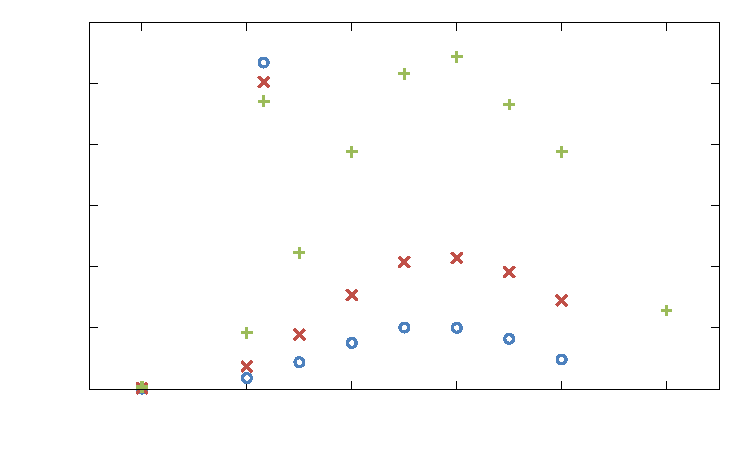
\includegraphics{GRAPH_Mag_vs_galaxies_in_time_JWST}}%
    \gplfronttext
  \end{picture}%
\endgroup

					}\endgroup
			\caption{Number of galaxies expected for different magnitudes, given set overall observing time (JW 6--8.5).\label{fig:galaxies_expected_JWST_6-8}}
		\end{figure}

		The results show clearly that for any survey time, the most beneficial survey depth is around magnitude 30 as it yields the most galaxies between redshift 6 and 8.5 (Figure~\ref{fig:galaxies_expected_JWST_6-8}). For a survey of 0.5\,million seconds total, magnitude 30 produces the best results, and for a survey of 0.1\,million seconds, approximately 100 galaxies would be expected at both magnitudes 29.5 and 30. This can be seen more clearly in Figure~\ref{fig:galaxies_expected_JWST_errors} which plots only the data for 0.1\,million seconds, but also includes error bars due to cosmic variance.
		\begin{figure}[!htbp]
			\centering
				\begingroup\endlinechar=-1
					\resizebox{0.8\textwidth}{!}{%
						% GNUPLOT: LaTeX picture with Postscript
\begingroup
  \makeatletter
  \providecommand\color[2][]{%
    \GenericError{(gnuplot) \space\space\space\@spaces}{%
      Package color not loaded in conjunction with
      terminal option `colourtext'%
    }{See the gnuplot documentation for explanation.%
    }{Either use 'blacktext' in gnuplot or load the package
      color.sty in LaTeX.}%
    \renewcommand\color[2][]{}%
  }%
  \providecommand\includegraphics[2][]{%
    \GenericError{(gnuplot) \space\space\space\@spaces}{%
      Package graphicx or graphics not loaded%
    }{See the gnuplot documentation for explanation.%
    }{The gnuplot epslatex terminal needs graphicx.sty or graphics.sty.}%
    \renewcommand\includegraphics[2][]{}%
  }%
  \providecommand\rotatebox[2]{#2}%
  \@ifundefined{ifGPcolor}{%
    \newif\ifGPcolor
    \GPcolortrue
  }{}%
  \@ifundefined{ifGPblacktext}{%
    \newif\ifGPblacktext
    \GPblacktexttrue
  }{}%
  % define a \g@addto@macro without @ in the name:
  \let\gplgaddtomacro\g@addto@macro
  % define empty templates for all commands taking text:
  \gdef\gplbacktext{}%
  \gdef\gplfronttext{}%
  \makeatother
  \ifGPblacktext
    % no textcolor at all
    \def\colorrgb#1{}%
    \def\colorgray#1{}%
  \else
    % gray or color?
    \ifGPcolor
      \def\colorrgb#1{\color[rgb]{#1}}%
      \def\colorgray#1{\color[gray]{#1}}%
      \expandafter\def\csname LTw\endcsname{\color{white}}%
      \expandafter\def\csname LTb\endcsname{\color{black}}%
      \expandafter\def\csname LTa\endcsname{\color{black}}%
      \expandafter\def\csname LT0\endcsname{\color[rgb]{1,0,0}}%
      \expandafter\def\csname LT1\endcsname{\color[rgb]{0,1,0}}%
      \expandafter\def\csname LT2\endcsname{\color[rgb]{0,0,1}}%
      \expandafter\def\csname LT3\endcsname{\color[rgb]{1,0,1}}%
      \expandafter\def\csname LT4\endcsname{\color[rgb]{0,1,1}}%
      \expandafter\def\csname LT5\endcsname{\color[rgb]{1,1,0}}%
      \expandafter\def\csname LT6\endcsname{\color[rgb]{0,0,0}}%
      \expandafter\def\csname LT7\endcsname{\color[rgb]{1,0.3,0}}%
      \expandafter\def\csname LT8\endcsname{\color[rgb]{0.5,0.5,0.5}}%
    \else
      % gray
      \def\colorrgb#1{\color{black}}%
      \def\colorgray#1{\color[gray]{#1}}%
      \expandafter\def\csname LTw\endcsname{\color{white}}%
      \expandafter\def\csname LTb\endcsname{\color{black}}%
      \expandafter\def\csname LTa\endcsname{\color{black}}%
      \expandafter\def\csname LT0\endcsname{\color{black}}%
      \expandafter\def\csname LT1\endcsname{\color{black}}%
      \expandafter\def\csname LT2\endcsname{\color{black}}%
      \expandafter\def\csname LT3\endcsname{\color{black}}%
      \expandafter\def\csname LT4\endcsname{\color{black}}%
      \expandafter\def\csname LT5\endcsname{\color{black}}%
      \expandafter\def\csname LT6\endcsname{\color{black}}%
      \expandafter\def\csname LT7\endcsname{\color{black}}%
      \expandafter\def\csname LT8\endcsname{\color{black}}%
    \fi
  \fi
  \setlength{\unitlength}{0.0500bp}%
  \begin{picture}(7200.00,4320.00)%
    \gplgaddtomacro\gplbacktext{%
      \put(747,595){\makebox(0,0)[r]{\strut{}-20}}%
      \put(747,986){\makebox(0,0)[r]{\strut{} 0}}%
      \put(747,1377){\makebox(0,0)[r]{\strut{} 20}}%
      \put(747,1768){\makebox(0,0)[r]{\strut{} 40}}%
      \put(747,2159){\makebox(0,0)[r]{\strut{} 60}}%
      \put(747,2551){\makebox(0,0)[r]{\strut{} 80}}%
      \put(747,2942){\makebox(0,0)[r]{\strut{} 100}}%
      \put(747,3333){\makebox(0,0)[r]{\strut{} 120}}%
      \put(747,3724){\makebox(0,0)[r]{\strut{} 140}}%
      \put(747,4115){\makebox(0,0)[r]{\strut{} 160}}%
      \put(1353,409){\makebox(0,0){\strut{} 27}}%
      \put(2360,409){\makebox(0,0){\strut{} 28}}%
      \put(3367,409){\makebox(0,0){\strut{} 29}}%
      \put(4375,409){\makebox(0,0){\strut{} 30}}%
      \put(5382,409){\makebox(0,0){\strut{} 31}}%
      \put(6389,409){\makebox(0,0){\strut{} 32}}%
      \csname LTb\endcsname%
      \put(144,2355){\rotatebox{-270}{\makebox(0,0){\strut{}Number of Galaxies}}}%
      \csname LTb\endcsname%
      \put(3871,130){\makebox(0,0){\strut{}Magnitude ($M$)}}%
      \put(3871,4022){\makebox(0,0){\strut{}}}%
    }%
    \gplgaddtomacro\gplfronttext{%
    }%
    \gplbacktext
    \put(0,0){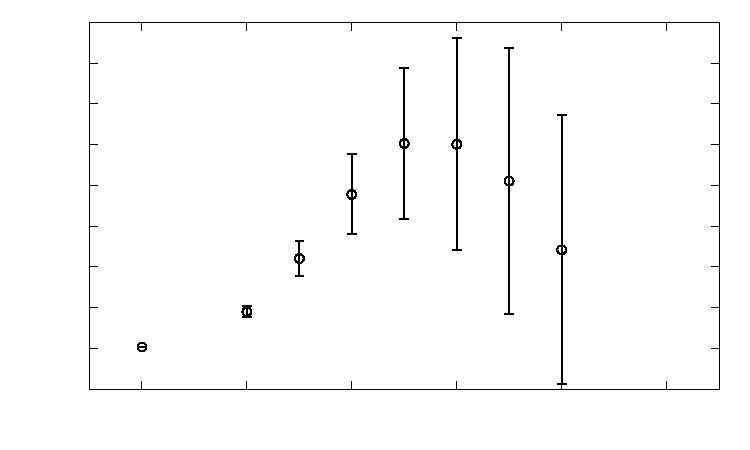
\includegraphics{GRAPH_Mag_vs_galaxies_in_time_JWST_01_errors}}%
    \gplfronttext
  \end{picture}%
\endgroup

					}\endgroup
			\caption{The number of galaxies observed given total observing time of 0.1\,million seconds, given different magnitude depths and resultantly different survey areas.\label{fig:galaxies_expected_JWST_errors}}
		\end{figure}

		It can be seen that the results for 29.5 and 30th magnitude predict very similar numbers of galaxies, however the error due to cosmic variance is significantly reduced for the 29.5\,magnitude due to the increased number of pointings at the sky, making it preferable. It was therefore decided that a survey with JWST, down to magnitude 29.5\,magnitude, with a total of 15 pointings, covering a total of 72.36\,square\,arc\,minutes would be used. This would take 0.1\,million seconds of open-shutter time for each filter.
	% subsection detailed_results_for_jwst (end)

	\subsubsection{Total Time for Survey} % (fold)
	\label{sub:total_time_for_survey}
		With each filter taking 0.1\,million seconds, and 3 filters needed to do colour analysis, the shutter will be open for around 0.3\,million seconds. On top of this are the overhead times, which as a crude approximation add an extra 10\% to take the time up to a total of 0.33\,million seconds. Given that the telescope can be operational for around 18\,hours per day, it is expected that the survey will take a minimum of 5.1\,days. Spectroscopy will be used to confirm the most promising candidates out of those observed using photometry, which will further add time to the survey.
	% subsection total_time_for_survey (end)
% section observing_strategy_for_redshift_6_8 (end)
